%!TeX root=../main.tex
\section{Model} % (fold)
\label{sec:model}

The structure of the data we consider, referred to as \emph{multivariate functional data}, is similar to that presented in \cite{happMultivariateFunctionalPrincipal2018a}. The data consist of independent trajectories of a vector-valued stochastic process $X = (\Xp{1}, \dots, \Xp{P})^\top$, $P\geq 1$. (Here and in the following, for any matrix $A$, $A^\top$ denotes its transpose.) For each $1 \leq p \leq P$, let $\TT{p}$ be a rectangle in some Euclidean space $\RR^{d_p}$ with $d_p \geq 1$, e.g., $\TT{p} = [0,1]^{d_p}$. Each coordinate $X^{(p)} : \TT{p} \rightarrow \RR$ is assumed to belong to  $\sLp{\TT{p}}$, the Hilbert space of square-integrable real-valued functions defined on $\TT{p}$, having the usual inner product that we denote by $\inLp{\cdot}{\cdot}$, and $\normLp{\cdot}$ the associated norm. Thus $X$ is a stochastic process indexed by $\pointt = (t_1, \ldots, t_P)$ belonging to the $P-$fold Cartesian product $\TT{} : =\TT{1} \times \cdots \times \TT{P}$ and taking values in the $P-$fold Cartesian product space $\HH \coloneqq \sLp{\TT{1}} \times \dots \times \sLp{\TT{P}}$. 

We consider the function $\inH{\cdot}{\cdot} : \HH \times \HH \rightarrow \RR$,
\begin{equation}\label{eq:innerprodH}
    \inH{f}{g} \coloneqq \sum_{p=1}^{P} \inLp{\fp}{\gp} = \sum_{p=1}^{P}\int_{\TT{p}} \fp(t_p)\gp(t_p) \dd t_p, \quad f, g \in \HH.
\end{equation}
$\HH$ is a Hilbert space with respect to the inner product $\inH{\cdot}{\cdot}$\citep{happMultivariateFunctionalPrincipal2018a}. We denote by $\normH{\cdot}$, the norm induced by $\inH{\cdot}{\cdot}$. Let $\mu : \TT{} \rightarrow \HH$ denote the mean function of the process $X$, $\mu(\pointt) \coloneqq \EE(X(\pointt)),\,\pointt \in \TT{}$. Let $C$ denote the $P \times P$ matrix-valued covariance function which, for $\points, \pointt \in \TT{}$, is defined as
\begin{equation}\label{eq:covariance_function}
    C(\points, \pointt) \coloneqq \EE\left(\{X(\points) - \mu(\points)\}\{X(\pointt) - \mu(\pointt)\}^{\top}\right), \quad \points, \pointt \in \TT{}.
\end{equation}
More precisely, for $1 \leq p, q \leq P$, the $(p, q)$th entry of the matrix $C(\points, \pointt)$ is the covariance function between the $p$th and the $q$th features of the process $X$:
\begin{equation}\label{eq:covariance_function_components}
    C_{p, q}(s_p, t_q) \coloneqq \EE\left(\{\Xp{p}(s_p) - \mup{p}(s_p)\}\{\Xp{q}(t_q) - \mup{q}(t_q)\}\right), \quad s_p \in \TT{p}, t_q \in \TT{q}.
\end{equation}
Let $\Gamma : \HH \rightarrow \HH$ denote the covariance operator of $X$, defined as an integral operator with kernel $C$. That is, for $f \in \HH$ and $\pointt \in \TT{}$, the $p$th feature of $\Gamma f(\pointt)$ is given by
\begin{equation}\label{eq:covariance_operator_components}
    (\Gamma f)^{(p)}(t_p) \coloneqq \inH{C_{p, \cdot}(t_p, \cdot)}{f(\cdot)} = \inH{C_{\cdot, p}(\cdot, t_p)}{f(\cdot)}, \quad t_p \in \TT{p}.
\end{equation}

Let us consider a set of $N$ curves $\XX = \{X_1, \ldots, X_n, \ldots, X_N\}$ generated as a random sample of the $P$-dimensional stochastic process $X$ with continuous trajectories. Unless otherwise stated, the data are assumed to be observed without error. The data can be viewed as a table with $N$ rows and $P$ columns where each entry is a curve, potentially on a multidimensional domain (see Figure~\ref{fig:data_matrix}). Each row of this matrix represents an observation; while each column represents a functional feature. At the intersection of row $n$ and column $p$, we thus have $\Xnp$ which is the curve that concerns the (functional) feature $p$ for the individual $n$.

\begin{figure}
    \centering
    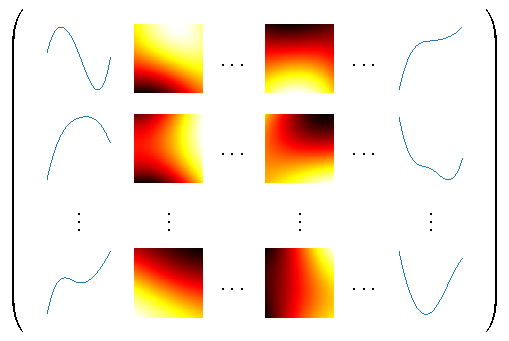
\includegraphics[]{figures/data_matrix.pdf}
    \caption{Functional data matrix, adapted from \cite{berrenderoPrincipalComponentsMultivariate2011}.}
    \label{fig:data_matrix}
\end{figure}

For $n \in \{1, \dots, N\}$, each observation $n$ is attributed the weight $\pi_n$ such that $\sum_n \pi_n = 1$, e.g., $\pi_n = 1/N$.
For a given $p \in \{1, \dots, P\}$, the mean curve of the $p$th feature along the $N$ observations is denoted by $\mup{p}$. This quantity can be computed as 
\begin{equation*}\label{eq:mu_estimation}
    \mup{p}(t_p) = \sum_{n = 1}^N \pi_n\Xnp(t_p), \quad t_p \in \TT{p}, \quad p \in \{1, \dots, P\}.
\end{equation*}
\add{The cross-covariance function of the $p$th and $q$th features along the $N$ observations can be computed as, for $p = 1, \dots, P$ and $q = 1, \dots, P$,
\begin{equation}\label{eq:cov_estimation}
    C_{p, q}(s_p, t_q) = \sum_{n = 1}^N \pi_n\Xnp(s_p)\Xnq(t_q) - \mup{p}(s_p)\mup{q}(t_q), \quad s_p \in \TT{p}, \quad t_q \in \TT{q}.
\end{equation}
}
For the set $\mathcal{X}$, the inner-product matrix, also called the Gram matrix, $M$ is defined as a matrix of size $N \times N$ with entries
\begin{equation}\label{eq:gram_mat}
    M_{nn^\prime} = \inH{X_n - \mu}{X_{n^\prime} - \mu}, \quad n, n^\prime = 1, \dots, N.
\end{equation}

\subsection{Basis decomposition} % (fold)
\label{sub:basis_decomposition}

% subsection basis_decomposition (end)

In many practical situations, functional data are noisy and only observed at specific time points. To extract the underlying functional features of the data, smoothing and interpolation techniques are commonly employed. These techniques involve approximating the true underlying function generating the data by a finite-dimensional set of basis functions. Assume that for each feature $p = 1, \dots, P$, there exists a set of basis of functions $\Psi^{(p)} = \{\psi_k^{(p)}\}_{1 \leq k \leq K_p}$ such that each feature of each curve $n = 1, \dots, N$ can be expanded using the basis:
\begin{equation}\label{eq:curve_basis_expansion}
\Xnp(t_p) = \sum_{k = 1}^{K_p} c^{(p)}_{nk}\psi_k^{(p)}(t_p), \quad t_p \in \TT{p},
\end{equation}
where $\{c^{(p)}_{nk}\}_{1 \leq k \leq K_p}$ is a set of coefficients for feature $p$ of observation $n$. We denote by $\overline{c}_k^{(p)} = \sum_{n = 1}^N \pi_n c^{(p)}_{nk}$ the mean coefficient of feature $p$ corresponding to the $k$th basis function.
The $p$th feature of the mean function can be then expanded in the same basis as:
\begin{equation}
    \mup{p}(t_p) = \sum_{k = 1}^{K_p} \overline{c}_k^{(p)}\psi_k^{(p)}(t_p), \quad t_p \in \TT{p}.
\end{equation}
In a similar way, the covariance function of the $p$th feature is given by:
\begin{equation}
    C_{p,p}(s_p, t_p) = \sum_{k = 1}^{K_p} \sum_{l = 1}^{K_p} \left(\sum_{n = 1}^N \pi_n c^{(p)}_{nk}c^{(p)}_{nl} - \overline{c}_k^{(p)}\overline{c}_l^{(p)}\right)\psi_k^{(p)}(s_p)\psi_l^{(p)}(t_p), \quad s_p, t_p \in \TT{p}.
\end{equation}
These formula can be written in matrix form as follows. For $\pointt \in \TT{}$, we have that $X(\pointt) = \mathbf{C}\Psi(\pointt)$ where $X(\pointt)$ is a $N \times P$ matrix with entries $\Xnp(t_p),~t_p \in \TT{p},~1 \leq p \leq P,~1 \leq n \leq N$,
\begin{equation}
    \mathbf{C} = \begin{pmatrix}
            \mathbf{C}^{(1)} & \cdots & \mathbf{C}^{(P)} \\
        \end{pmatrix}, \quad \text{and}\quad
    \Psi(\pointt) = \text{diag}\{\Psi^{(1)}(t_1), \dots, \Psi^{(P)}(t_P)\},
\end{equation}
where
\begin{equation}
\mathbf{C}^{(p)} = \begin{pmatrix}
    c^{(p)}_{11} & \cdots & c^{(p)}_{1K_p} \\
    \vdots & \ddots & \vdots \\
    c^{(p)}_{N1} & \cdots & c^{(p)}_{NK_p}
\end{pmatrix} \\
\quad \text{and}\quad
\Psi^{(p)}(t_p) = \begin{pmatrix}
    \psi_1^{(p)}(t_p) \\
    \vdots \\
    \psi_{K_p}^{(p)}(t_p)
\end{pmatrix}.
\end{equation}
Using the basis expansion and denoting $\Pi^\top = (\pi_1, \dots, \pi_N)$, the mean and covariance functions are given by
\begin{equation}
    \mu(\pointt) = \Psi(\pointt)^\top \mathbf{C}^\top\Pi \quad\text{and}\quad C(\points, \pointt) = \Psi(\points)^\top \mathbf{C}^\top \left(\text{diag}\{
        \pi_1, \dots, \pi_N\} - \Pi\Pi^\top\right)\mathbf{C} \Psi(\pointt).
\end{equation}
Finally, we denote by $\mathbf{W}$ the matrix of inner products of the functions in the basis $\Psi$. The matrix $\mathbf{W}$ is a block-diagonal matrix such that $\mathbf{W} = \text{diag}\{\mathbf{W}^{(1)}, \dots, \mathbf{W}^{(P)}\}$ where each entry is given by
\begin{equation}
    \mathbf{W}_{k, l}^{(p)} = \inLp{\psi_k^{(p)}}{\psi_l^{(p)}}, \quad 1 \leq k, l \leq K_p, \quad 1 \leq p \leq P.
\end{equation}
We remark that, if the basis $\Psi$ is an orthonormal basis, the matrix $\mathbf{W}$ is equal to the identity matrix of size $\sum_{p = 1}^P K_p$.
Using the expansion of the data into the basis of functions $\Psi$, the inner-product matrix $\mathbf{M}$ is written 
\begin{align}
    \mathbf{M} &= \left(\mathrm{I}_{\!N} - \mathbf{1}_{\!N}\Pi^\top\right) \mathbf{C} \mathbf{W} \mathbf{C}^\top \left(\mathrm{I}_{\!N} - \Pi\mathbf{1}_{\!N}^\top\right) \\
      &= \left[\left(\mathrm{I}_{\!N} - \mathbf{1}_{\!N}\Pi^\top\right)\mathbf{C}\mathbf{W}^{1/2}\right]\left[\left(\mathrm{I}_{\!N} - \mathbf{1}_{\!N}\Pi^\top\right)\mathbf{C}\mathbf{W}^{1/2}\right]^\top,
\end{align}
where $\mathrm{I}_{\!N}$ is the identity matrix of size $N$ and $\mathbf{1}_{\!N}$ is a vector of $1$ of length $N$.


% section model (end)